\documentclass{beamer}

\usepackage[utf8]{inputenc}
\usepackage[brazil]{babel}
\usepackage{graphicx}
\usepackage{adjustbox}

\usetheme{Madrid}
\usecolortheme{lily}

\definecolor{myNewColorA}{rgb}{0, 0, 100}
 \definecolor{blue(pigment)}{rgb}{0.2, 0.2, 0.6}
\setbeamercolor{titlelike}{parent=structure, bg=blue(pigment), fg=white}


%Information to be included in the title page:
\title[A radiação ultravioleta] %optional
	{Um protótipo de um medidor de índice de radiação ultravioleta}
 
\author% (optional, for multiple authors)
{ C. S. Gonçalves\and J. M. Reinoso \and J. N. B. Paiva \and S. T. S. Sousa \\ A. P. Carmo \and F. A. T. Campos}
 
\institute[IFF - Campus Cabo Frio] % (optional)
{

  Instituto Federal Fluminense\\
  Cabo Frio
  
}
 
\date{07 de Dezembro de 2019}

\begin{document}	

	\frame{\titlepage} 
	
	
	\AtBeginSection[]{
  	\begin{frame}
    	\frametitle{Sumário}
    	\tableofcontents[currentsection]
  	\end{frame}
	}

	\begin{frame}
		\frametitle{Objetivos}
		\begin{itemize}
			\item Definir o que é a radiação ultravioleta;
			\item Falar sobre o índice de radiação ultravioleta e sua importância;
			\item Descrever o protótipo do medidor de índice de radiação ultravioleta.
		\end{itemize}

	\end{frame}
		
	
	\section{Introdução}
	\begin{frame}
		\frametitle{O que é a radiação ultravioleta?}
			
		\begin{columns}
			\column{0.60\textwidth}
			\begin{itemize}
				\item Faz parte do espectro eletromagnético;
				\item Temos o UVA, UVB e UVC;
				\item Exposições prolongadas à radiação ultravioleta podem provocar danos ao ser humano.
			\end{itemize}

			\column{0.35\textwidth}
			\begin{figure}[htb]
				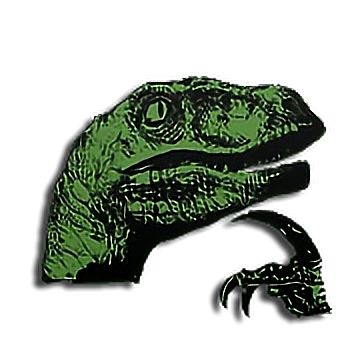
\includegraphics[width=0.95\textwidth]{img/dino.png}
			\end{figure}

		\end{columns}
		
	\end{frame}
	
	\begin{frame}
	\frametitle{O que é a radiação?}	
		\begin{columns}
			\column{.5\textwidth}
			Radiação é a emissão de energia de uma fonte.
			\column{.5\textwidth}
			\begin{figure}[htb]
				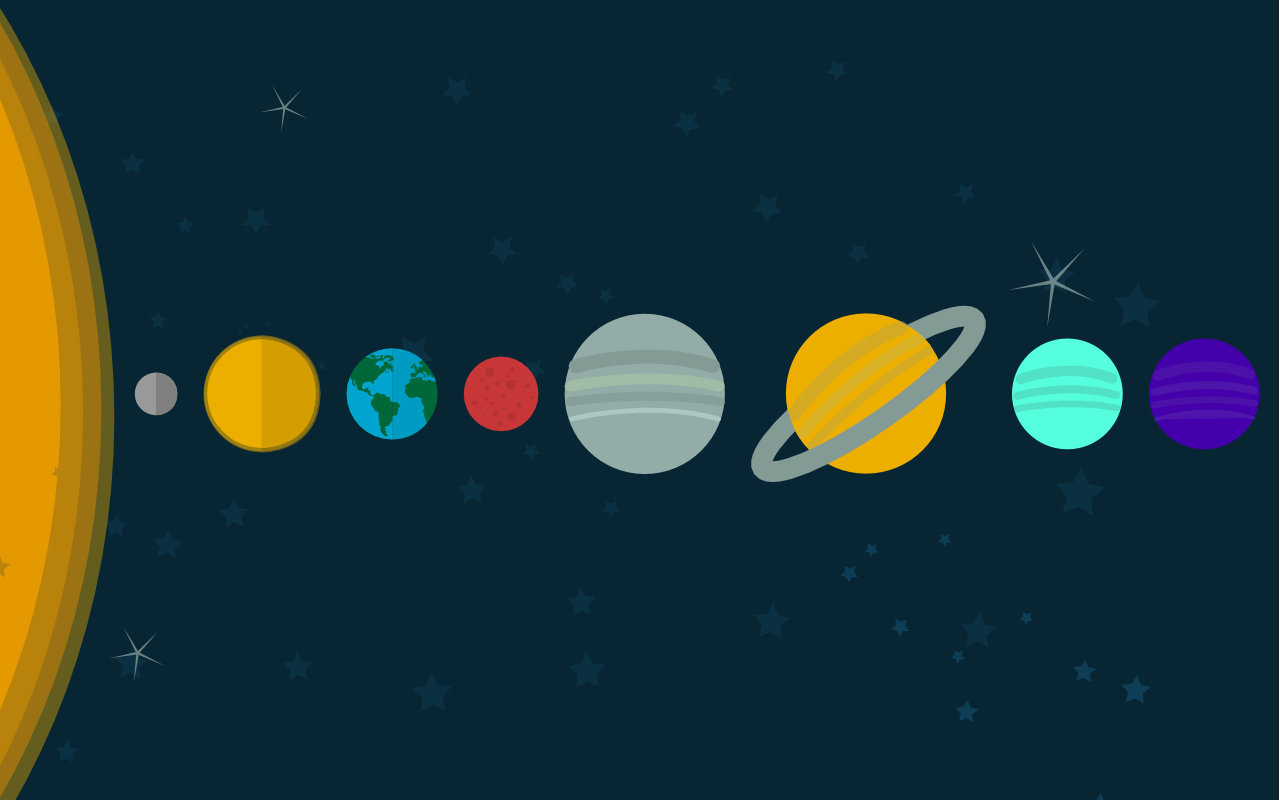
\includegraphics[width=0.95\textwidth]{img/sistema-solar.png}
				\caption{O Sol é uma grande fonte de energia}
			\end{figure}
	
		\end{columns}	
		
	\end{frame}
	
	\begin{frame}
		\frametitle{O que é a radiação ultravioleta?}	
		\begin{columns}
			\column{.5\textwidth}
				Há vários tipo de radiação, variando de altas frequências, com maiores energias, até frequências mais baixas, apresentando 
				menores quantidades de energia. Tem mais energia que a luz visível e menos que os raios-X.
			
			\column{.5\textwidth}
			\begin{figure}[htb]
				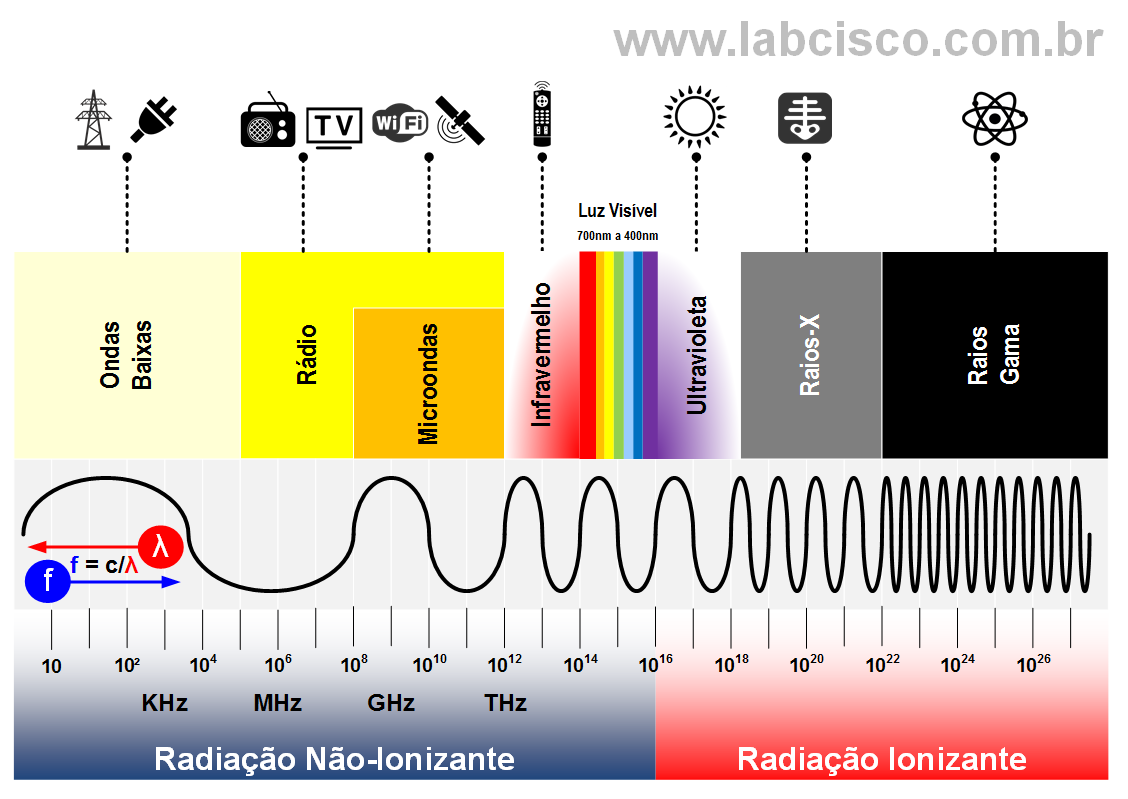
\includegraphics[width=0.95\textwidth]{img/espectro_eletromagnetico.png}
				\caption{O espectro eletromagnético}
			\end{figure}
					
		\end{columns}
	\end{frame}
	
	
	\begin{frame}
		\frametitle{UVA, UVB e UVC} 
			\begin{figure}[htb]
				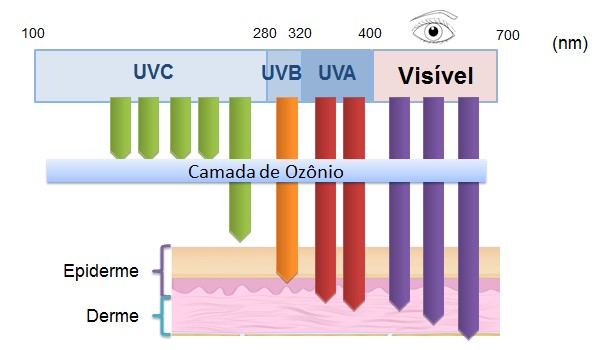
\includegraphics[width=0.95\textwidth]{img/uvlight_spectrum1.jpg}
				\caption{Os intervalos da radiação ultravioleta}
			\end{figure}	
	\end{frame}
	
	\begin{frame}
		\frametitle{Raios UVA e UVB e os danos} 
			\begin{figure}[htb]
				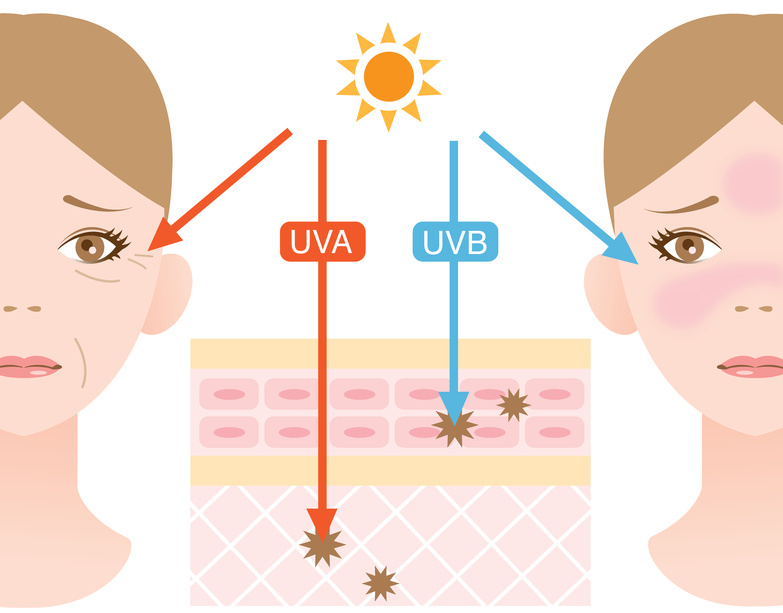
\includegraphics[width=0.70\textwidth]{img/raio_uva_uvb.jpg}
				\caption{Exposições prolongadas ao sol e sem proteção solar}
			\end{figure}
			
	\end{frame}
	
	
	\section{O índice de radiação ultravioleta}
		\begin{frame}
			\frametitle{O índice de radiação UV} 
			\begin{itemize}
				\item O índice de radiação solar descreve a intensidade da radiação ultravioleta na superfície da Terra;
				\item Esse parâmetro tem o objetivo de alertar as pessoas os danos que a radiação ultravioleta pode trazer, caso a exposição a ela seja duradoura;
				\item A cada índice de radiação ultravioleta mensurado, há medidas de proteções a serem tomadas.
			\end{itemize}
		\end{frame} 
			
			
		\begin{frame}
			\frametitle{O índice de radiação UV} 
				\begin{figure}[htb]
					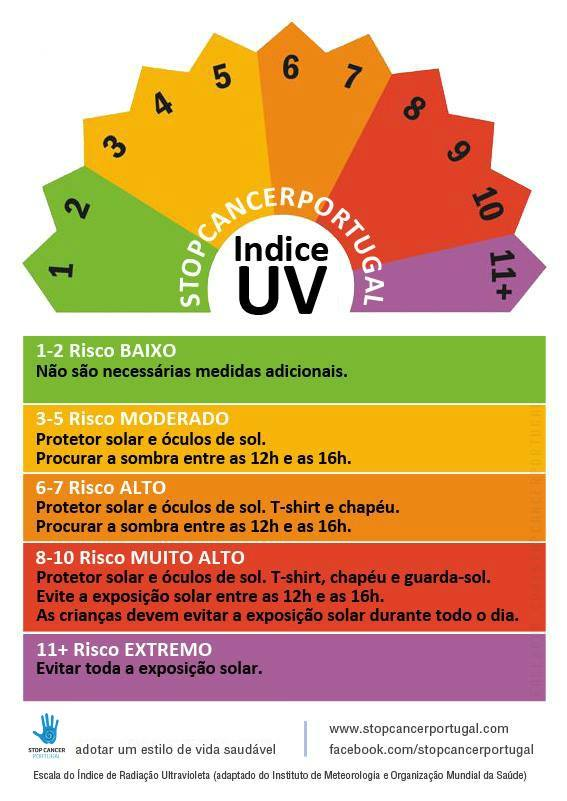
\includegraphics[width=0.40\textwidth]{img/Tabela-UV.jpg}
					\caption{O índice de radiação ultravioleta e as precauções}
				\end{figure}
			\end{frame}
			
			\begin{frame}
			\frametitle{O índice de radiação UV} 
				\begin{figure}[htb]
					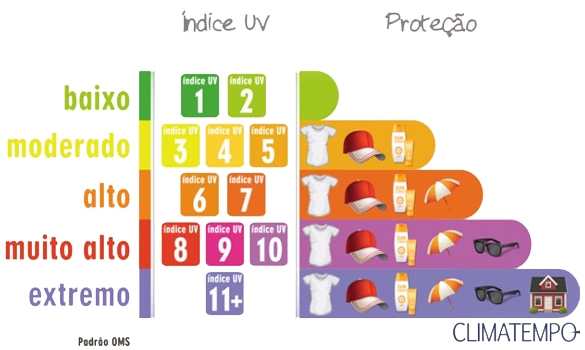
\includegraphics[width=0.75\textwidth]{img/Tabela-UV-2.jpg}
					\caption{O índice de radiação ultravioleta e as precauções}
				\end{figure}
			\end{frame}
	
	\section{O protótipo}
	
	
	\begin{frame}
		\frametitle{O microcontrolador}
		\begin{figure}[htb]
					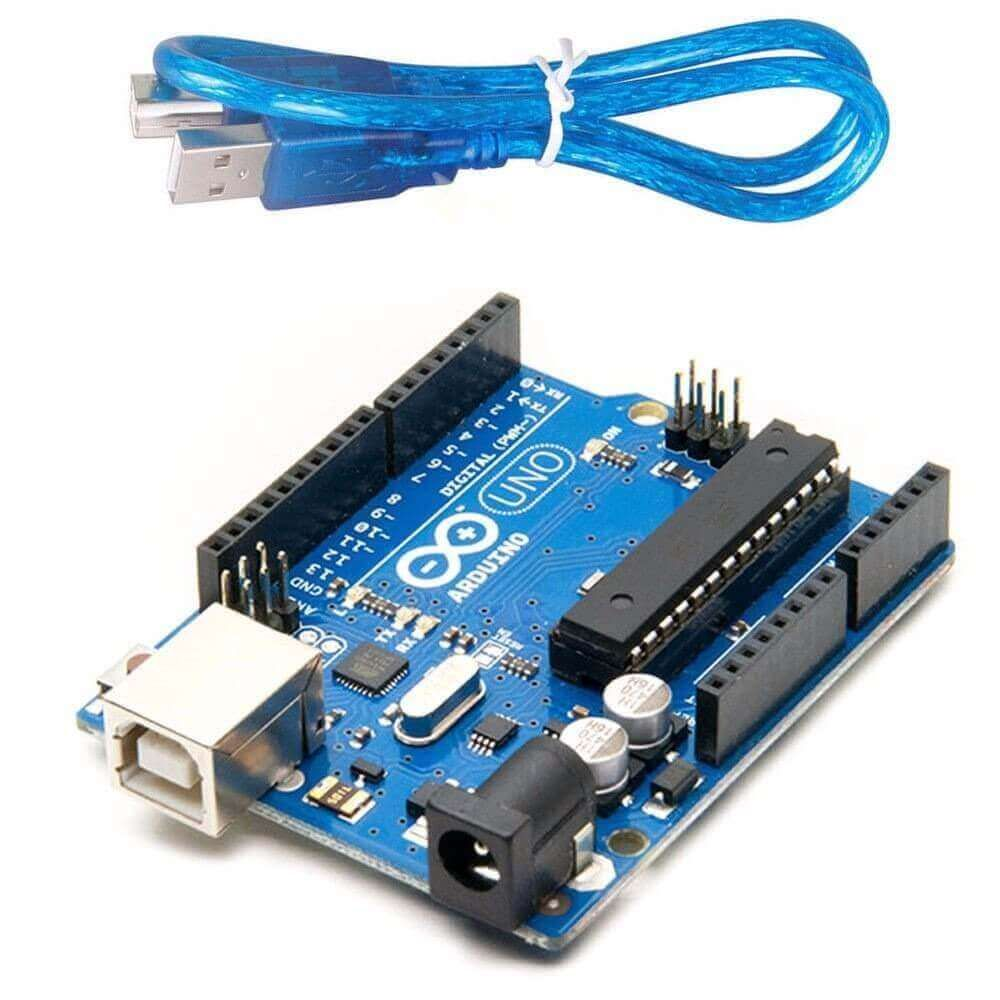
\includegraphics[width=0.5\textwidth]{img/arduino.jpg}
					\caption{Um placa Arduíno Uno}
				\end{figure}
	\end{frame}
	
	
	\begin{frame}
		\frametitle{Sensores}
		\begin{columns}
			\column{0.45\textwidth}
				\begin{figure}[htb]
					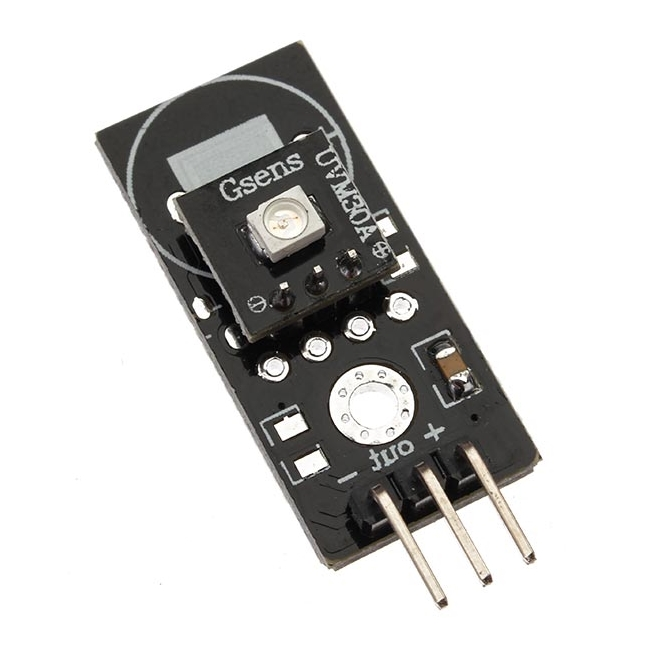
\includegraphics[width=0.8\textwidth]{img/sensor_uvma.jpg}
					\caption{Sensor de radiação ultravioleta UVM -30A}
				\end{figure}
				
			\column{0.45\textwidth}
				\begin{figure}[htb]
					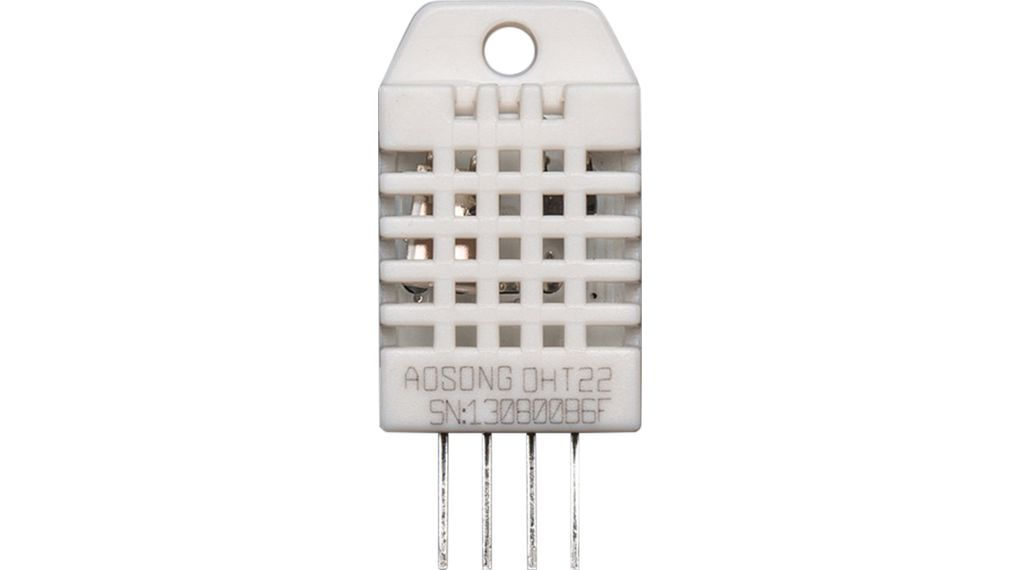
\includegraphics[width=0.8\textwidth]{img/sensor_dht22.jpg}
					\caption{Sensor de umidade e temperatura DHT22}
				\end{figure}
		\end{columns}
				
	\end{frame}
	
	
	\begin{frame}
		\frametitle{Um módulo RTC}
		\begin{figure}[htb]
					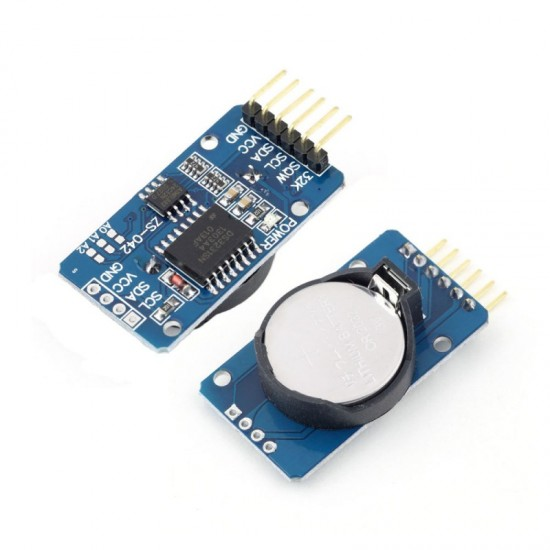
\includegraphics[width=0.5\textwidth]{img/rtc.jpg}
					\caption{Módulo Real Time Clock DS3231 }
				\end{figure}
	\end{frame}
	
	\begin{frame}
		\frametitle{LEDS}
		\begin{figure}[htb]
					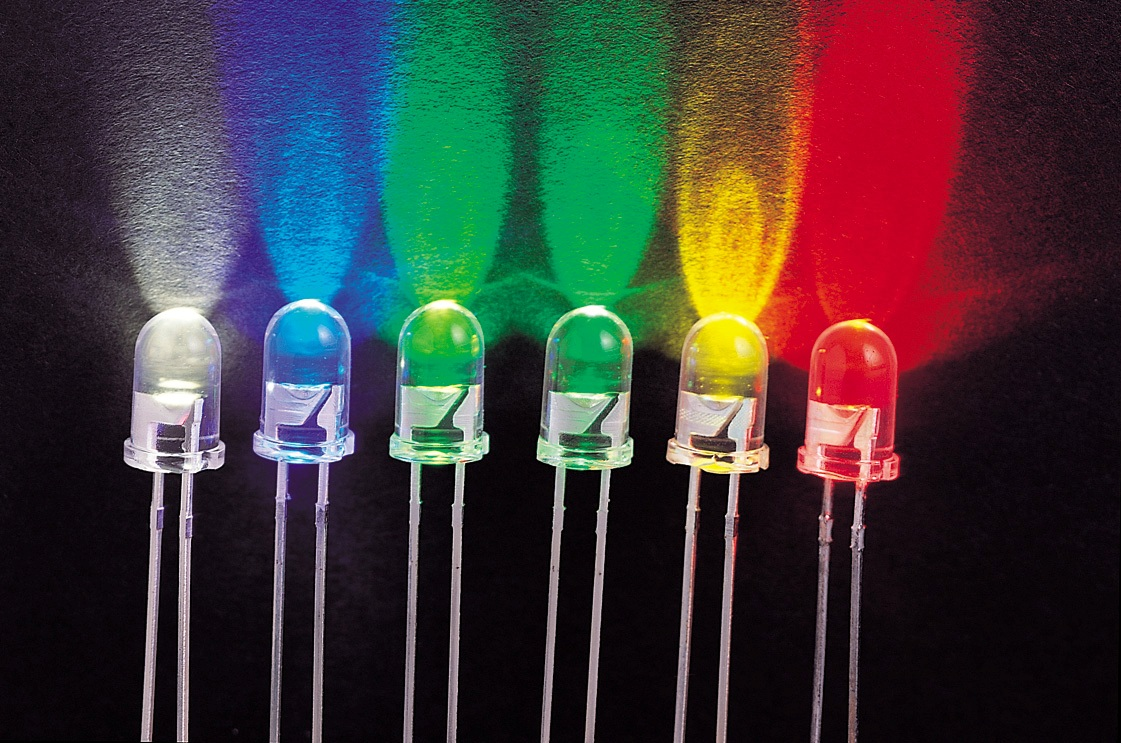
\includegraphics[width=0.8\textwidth]{img/leds.jpg}
					\caption{Alguns leds serão necessários}
				\end{figure}
	\end{frame}
	
	\begin{frame}
		\frametitle{Display}
		\begin{figure}[htb]
					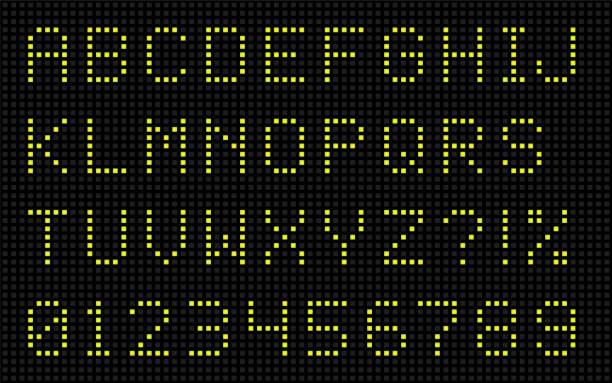
\includegraphics[width=0.8\textwidth]{img/display.jpg}
					\caption{Um LED, um pixel....}
				\end{figure}
	\end{frame}

	\begin{frame}
		\frametitle{Um esboço do projeto}
		\begin{figure}[htb]
					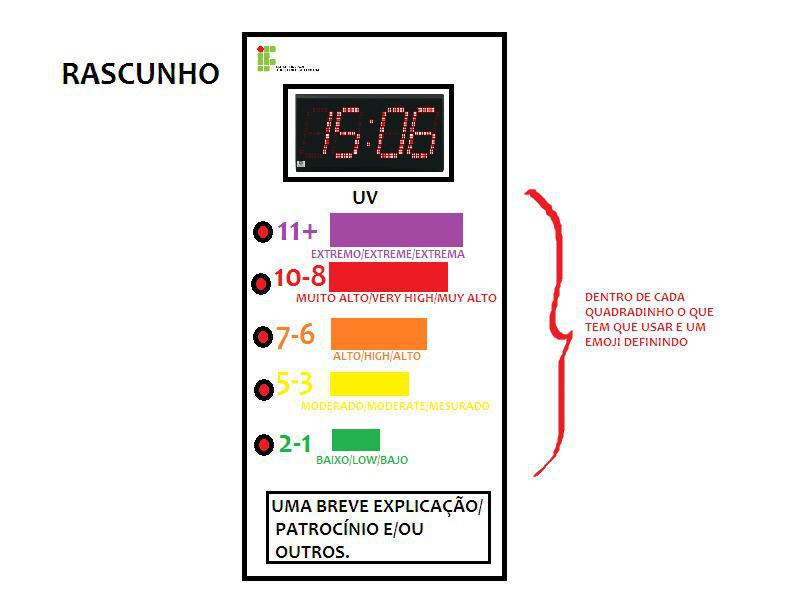
\includegraphics[width=0.8\textwidth]{img/toten_prot.jpg}
				\end{figure}
	\end{frame}
	
	\section{Conclusões}
	\begin{frame}
		\frametitle{Conclusões}
		\begin{itemize}
			\item A exposição excessiva à radiação ultravioleta pode trazer graves riscos à saúde do ser humano;
			\item O índice de radiação ultravioleta traz as informações necessárias de como as pessoas devem agir mediante a níveis de radiação ultravioleta;
			\item O protótipo fará o uso das informações referentes ao índice de radiação ultravioleta para conscientizar as pessoas locais sobre a radiação ultravioleta.
		\end{itemize}

	\end{frame}
	
	\begin{frame}
		\frametitle{Agradecimentos}
		Agradecimentos ao Instituto Federal Fluminense, campus Cabo Frio e ao CNPQ pelo auxílio financeiro.
		\begin{columns}
			\column{0.45\textwidth}
				\begin{figure}[htb]
					
\includegraphics[width=0.8\textwidth]{img/iff.png}
				\end{figure}
				
			\column{0.45\textwidth}
				\begin{figure}[htb]
					
\includegraphics[width=0.8\textwidth]{img/cnpq.png}
				\end{figure}
		\end{columns}

	\end{frame}


	\section*{Referências}
		\begin{frame}
		\frametitle{Obrigado pela atenção!!}
			\begin{figure}[htb]
				
\includegraphics[width=0.95\textwidth]{img/obrigado.jpg}
			\end{figure}
		\end{frame}
	
	
\end{document}